\begin{figure}[H]
    \begin{subfigure}{0.32\textwidth}
        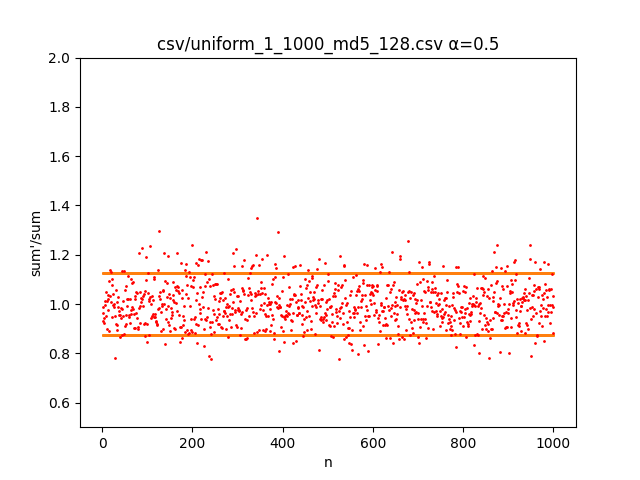
\includegraphics[width=1.0\linewidth, height=5cm]{czebyszew/uniform_1_1000_md5_128_m_128_a_0_5.png}
        \caption{$\alpha = 0.5$}
        \label{fig:subim2}
    \end{subfigure}
    \begin{subfigure}{0.32\textwidth}
        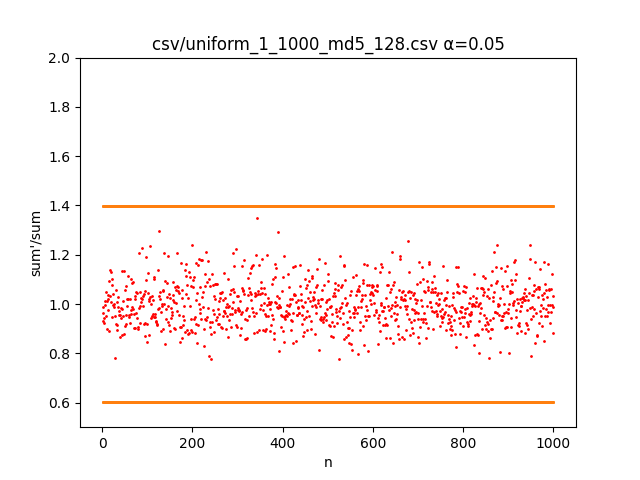
\includegraphics[width=1.0\linewidth, height=5cm]{czebyszew/uniform_1_1000_md5_128_m_128_a_0_05.png}
        \caption{$\alpha = 0.05$}
        \label{fig:subim2}
    \end{subfigure}
    \begin{subfigure}{0.32\textwidth}
        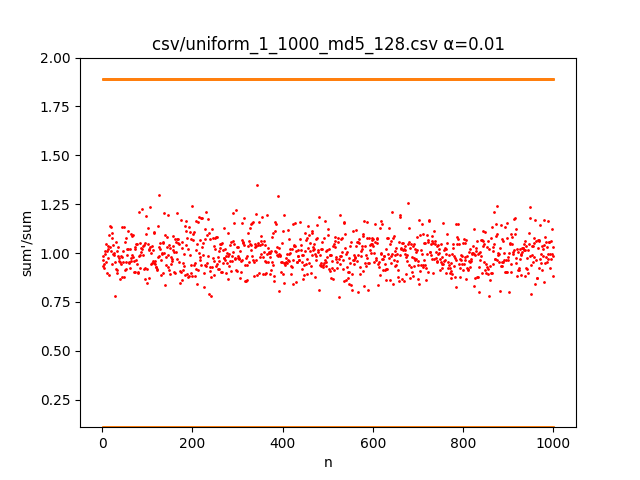
\includegraphics[width=1.0\linewidth, height=5cm]{czebyszew/uniform_1_1000_md5_128_m_128_a_0_01.png}
        \caption{$\alpha = 0.1$}
        \label{fig:subim2}
    \end{subfigure}

    \caption{Wykresy przedstawiają nierówności Czebyszewa nałożone na wykresy z różnymi parametrami $\alpha$. Możemy zaobserwować, że ograniczenia uzyskane z nierówności prawidłowo odzwierciedlają otrzymane wyniki.}
    \label{fig:uniform_md5}
\end{figure}